% 12pt .6pt grayscale native fragment
\usetikzlibrary{calc}
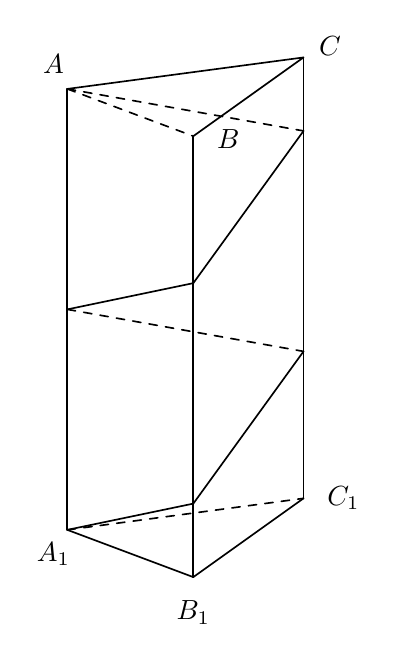
\begin{tikzpicture}[line width=0.6pt, line join=round, line cap=round, >=stealth]
\tikzset{hid/.style={dashed}}
\coordinate (A) at (0,5.6); \coordinate (B) at (1.6,5.0); \coordinate (C) at (3.0,6.0);
\coordinate (A1) at (0,0); \coordinate (B1) at (1.6,-0.6); \coordinate (C1) at (3.0,0.4);
\draw (A)--(A1); \draw (B)--(B1); \draw (C)--(C1);
\draw (A)--(C)--(B); \draw[hid] (A)--(B);
\draw (A1)--(B1)--(C1); \draw[hid] (A1)--(C1);
\draw[dashed] (0,5.6)--(3,5.066666667);
\draw (3,5.066666667)--(1.6,3.133333333);
\draw (1.6,3.133333333)--(0,2.8);
\draw[dashed] (0,2.8)--(3,2.266666667);
\draw (3,2.266666667)--(1.6,0.3333333333);
\draw (1.6,0.3333333333)--(0,0);
\node[left=5pt,above=2pt] at (A) {$A$}; \node[below=1pt,right=5pt] at (B) {$B$}; \node[above=4pt,right=2pt] at (C) {$C$};
\node[left=5pt,below=1pt] at (A1) {$A_{1}$}; \node[below=5pt] at (B1) {$B_{1}$}; \node[right=5pt] at (C1) {$C_{1}$};
\end{tikzpicture}
